%! TeX program = lualatex
% při kompilaci dokumentu LuaLaTeXem dojde k chybě, protože
% nedefinuje \pdfpagewidth a \pdfpageheight. 
% Balíček luatex85 to napravuje
\ifdefined\directlua
\RequirePackage{luatex85}
\fi

\documentclass{ltugboat}
% \usepackage[T1]{fontenc}
% \usepackage[utf8]{inputenc}
\usepackage{fontspec}
\setmainfont[Ligatures={TeX,Rare}]{Latin Modern Roman}
\usepackage[czech,english]{babel}
\usepackage{luavlna}
\usepackage[noautomatic]{responsive}
\usepackage{lua-widow-control}
\usepackage{csquotes}
\usepackage{linebreaker}
\usepackage{amsmath,amsfonts}

\usepackage{graphicx}
\usepackage{caption}
\usepackage{subcaption}
\usepackage{lipsum}


% \usepackage[
%   backend=biber,
%   % style=iso-numeric,
%   style=numeric,
%   sortlocale=cs,
%   autolang=other,
%   bibencoding=UTF8,
%   mincitenames=2,
%   maxcitenames=2,
% ]{biblatex}
% \addbibresource{responsive.bib}
\usepackage[
  implicit=false,
  hidelinks,
]{hyperref}


\newcommand\program[1]{#1}

% pro případ, kdy je \lipsum moc velké 
\newcommand\smalllipsum{%
Lorem ipsum dolor sit amet,
consectetuer adipiscing elit.
Ut purus elit, vestibulum ut,
placerat ac, adipiscing vitae,
felis. Curabitur dictum gravida 
mauris. Nam arcu libero, nonummy 
eget, consectetuer id, vulputate 
a, magna. Donec vehicula augue eu neque.
}

\newcommand\printsize[1]{\csname #1\endcsname\par\noindent Sample\par}
\newcommand\showscale[2][.5\textwidth]{%
      % \setsizes[38]{25}
      \printsize{huge}
      \printsize{LARGE}
      \printsize{Large}
      \printsize{large}
      \hrule
      \printsize{normalsize}
      \hrule
      \printsize{small}
      \printsize{footnotesize}
}


\title{Responzivní design a automatická sazba s Lua\LaTeX em}

% repeat info for each author; comment out items that don't apply.
\author{Michal Hoftich}
\address{Magdalény Rettigové 4\\ Praha, 116 39\\ Czechia}
\netaddress{michal.h21 (at) gmail dot com}
\personalURL{https://www.kodymirus.cz/}
\begin{document}

\maketitle

\begin{abstract}
This article presents the use of responsive design methods and advanced features
of Lua\LaTeX\ for automatic document typesetting intended for various target outputs,
both printed and electronic, such as mobile phones, tablets, or e-readers.

Specifically, it focuses on the use of Lua\LaTeX\ for automated
typesetting with the help of the \tbcode{Responsive} package~\cite{responsive} for setting font size and line spacing
according to page size, the \tbcode{Luavlna} package~\cite{luavlna} to prevent single-character prepositions
at the ends of lines, the \tbcode{Lua-widow-control} package~\cite{lua-widow-control} to minimize widows and orphans at the ends and
beginnings of pages, and the \tbcode{Linebreaker} package~\cite{linebreaker} to prevent line overflow.

\end{abstract}


\section{Introduction}

Some time ago, I acquired an e-book reader, but I still read most texts on my
PC screen because they come from web sources. It occurred to me that I could
save longer articles for later reading on my e-reader. There are, of course,
several applications for this purpose, but I decided to create my own, tailored
exactly to my needs and preferences. Another motivation is the opportunity to
learn something new and create packages that will be useful for other \TeX\
users as well.

My goal is to make the solution as automated as possible, so I don't have to
deal with overflow lines or other errors that would require manual
intervention. Thanks to the capabilities of Lua\LaTeX, such a solution is
already possible, as we will demonstrate in the following text.

Because Lua\TeX\ includes the Lua programming language in \TeX\ distributions,
I used it to create my project \program{Rmodepdf} \cite{rmodepdf}. It uses the
\tbcode{LuaXML} package \cite{luaxml} to transform HTML into \TeX{} and the
\program{Curl} commands to download the page, \program{Tidy} to fix HTML
errors, and \program{Rdrview} \cite{rdrview}, which removes navigation
elements, advertisements, and other distractions from the page.
\program{Rdrview} works similarly to the reader mode in the \program{Firefox}
browser (illustrated in Figure~\ref{fig:readermode}).

However, in the following text, I will not focus on the \program{Rmodepdf}
program itself, which is still not in a state suitable for general users. I
believe that readers will find it more useful to describe the methods for
automated typesetting and responsive design, which they can use in typesetting
their own documents.

\begin{figure*}[tbp]
  \centering
  \caption{Example of using the \emph{reader view} mode in the \program{Firefox} browser}
  \label{fig:readermode}
  \begin{subfigure}[t]{0.45\textwidth}
    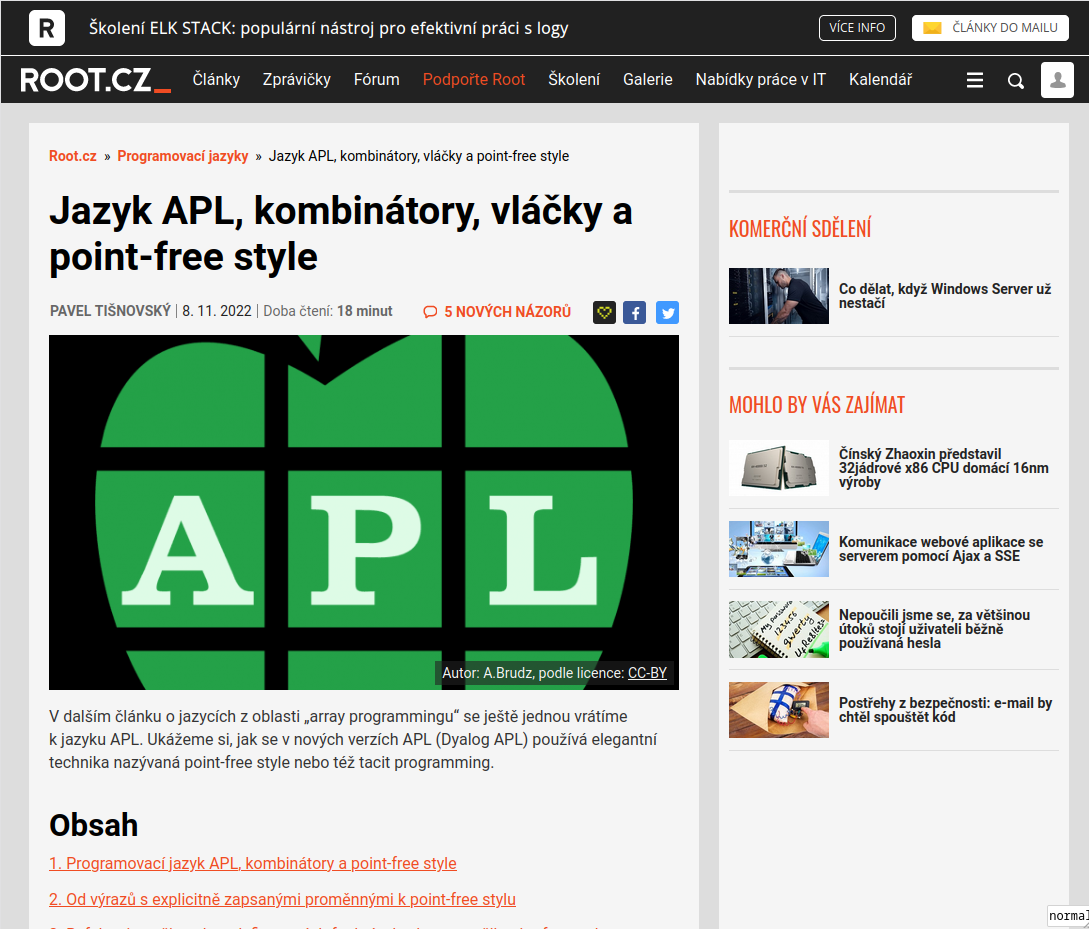
\includegraphics[width=\textwidth]{img/root-balast.png}
    \caption{Page with control elements and ads}
  \end{subfigure}
  \hfill
  \begin{subfigure}[t]{0.45\textwidth}
    \includegraphics[width=\textwidth]{img/root-čtečka.png}
    \caption{Page in reader view}
  \end{subfigure}
\end{figure*}

\section{How to Convert a Web Page to PDF Using \LaTeX}

% https://github.com/eafer/rdrview

\begin{verbatim}
$ rdrview -H <url> | pandoc -f html -t latex -V lang=cs \
  --template template.tex output.html > output.tex
\end{verbatim}


\section{Responsive Design}

One of the issues that need to be addressed is setting the correct font size
for readability. The default font size in \LaTeX\ is 10 points, regardless of
the page size. This is a suitable font size for an A5 page. For A4 format, the
font size should be larger, and for smaller screens of e-readers and mobile
phones, it can be smaller. Similarly, we can change the line spacing, which
also affects text readability depending on the font size and page size.

Web browsers face a similar problem, as they need to display text on large PC
monitors as well as on smaller screens of laptops, tablets, and mobile phones.
The solution they use is called \textit{responsive design}.

Responsive design is a way of designing web pages that allows flexible and
dynamic adaptation of the appearance and layout of the page content to
different display devices. One of the key elements of responsive design is a
flexible structure that allows elements on the page to be resized to fit the
display device.

Another important element is \textit{media queries}. These allow defining rules
that apply based on the properties of the display device, such as screen width
and height or the type of output (paper, display). Thanks to these rules, the
same page code can be well displayed on both large monitors and mobile devices
or when printed. An example of real-world use can be seen in
Figure~\ref{fig:responsive}.

\begin{figure*}[tbp]
\begin{subfigure}[t]{0.74\textwidth}
    
\includegraphics[width=\textwidth]{img/pedf-web-big.png}
    \caption{Example of a page on a large monitor}
\end{subfigure}
\hfill
\begin{subfigure}[t]{0.24\textwidth}
    \includegraphics[width=\textwidth]{img/pedf-web-small.png}
    \caption{Example of a page on a small display}
\end{subfigure}
  \caption{Example of displaying a web page using responsive design}\label{fig:responsive}
\end{figure*}

The \tbcode{Responsive} package~\cite{responsive} is inspired by these
principles. Its main function is to set the font size according to the page
size and the approximate number of characters that should fit on the page. It
also sets the typographic scale (affecting font sizes for headings or
footnotes), the font baseline, and supports a simple version of media queries.

\subsection{Setting up the \tbcode{Responsive} Package}

\tbcode{Responsive} automatically sets the font size, line spacing, and
typographic scale at the beginning of the document. Default values can be
changed using package options (\verb|\usepackage[<options>]{responsive}|) or
the \verb|\ResponsiveSetup{<options>}| command. The \verb|\ResponsiveSetup|
command can also be used directly in the document text, for example, for local
font settings changes.

The \tbcode{Responsive} package offers the following options:

\begin{description}
  \item[noautomatic] – prevents automatic setting of font size and line spacing at the beginning of the document.
  \item[characters] – number of characters for automatic font size setting.
  \item[scale] – typographic scale used for font sizes.
  \item[lineratio] – ratio used in line spacing calculation.
\end{description}

\subsection{Basic Font Size}

The font size can be set using the \verb|\setsizes{<number of characters per|\allowbreak\verb|line>}| 
command. \tbcode{Responsive} tries to set the font
size so that the desired number of characters fits on a line on average. The
actual number of characters depends on the text used, as each letter has a
different width when using proportional fonts. In reality, the number of
characters displayed on a line may be slightly higher.

If the number of characters is not specified in the \verb|\setsizes| command,
the value of the \texttt{characters} option is used. The following example uses
this option setting. Figure~\ref{fig:fontsize} shows how the same text can be
displayed differently within the same frame, depending on the settings.

\begin{verbatim}
\begin{minipage}{5cm}
\ResponsiveSetup{characters=55}
\setsizes{}
\lipsum[1]
\end{minipage}
\end{verbatim}

\begin{figure*}[tbp]
  \begin{subfigure}[t]{0.45\textwidth}
\fbox{%
\begin{minipage}{5cm}
\ResponsiveSetup{characters=55}
\setsizes{}

\lipsum[1]

\end{minipage}}
\caption{\texttt{characters=55}}
\end{subfigure}
\hfill
\begin{subfigure}[t]{0.45\textwidth}
\fbox{%
\begin{minipage}{5cm}
\ResponsiveSetup{lineratio=38,characters=25}
\setsizes{}

Lorem ipsum dolor sit amet,
consectetuer adipiscing elit.
Ut purus elit, vestibulum ut,
placerat ac, adipiscing vitae,
felis. Curabitur dictum gravida 
mauris. Nam arcu libero, nonummy 
eget, consectetuer id, vulputate 
a, magna. Donec vehicula augue eu neque.

\end{minipage}}
\caption{\texttt{characters=25, lineratio=38}}
\end{subfigure}
  \caption{Difference in font size depending on the number of characters per line}\label{fig:fontsize}
\end{figure*}

\subsection{Line Spacing}

By default, \LaTeX\ sets the line spacing to the font size multiplied by 1.2.
For different fonts and page sizes, a different line spacing may be
appropriate. Similarly, different values may be suitable for the printed and
electronic versions of the document.

I was inspired by Edoardo Cavazza's article~\cite{cavazza} on readability and
added support for setting line spacing based on the ratio of lowercase letter
height and the \texttt{lineratio} variable. This ratio is obtained by the
following calculation:

\[ \text{line spacing} = \frac{1\text{ex}}{\text{lineratio}/100} \]

You can observe the impact of changing the \texttt{lineratio} value in
Figure~\ref{fig:lineratio}. The choice of its optimal value depends on the font
used and the page size. To achieve maximum output readability, it's advisable
to compare the output using different values.

\begin{figure*}[tbp]
  \begin{subfigure}[b]{0.45\textwidth}
\fbox{%
\begin{minipage}{5cm}
\ResponsiveSetup{lineratio=38}
\setsizes{65}

\lipsum[1]

\end{minipage}}
\caption{\texttt{lineratio=38}}
\end{subfigure}
\begin{subfigure}[b]{0.45\textwidth}
\fbox{%
\begin{minipage}{5cm}
\ResponsiveSetup{lineratio=34}
\setsizes{65}

\lipsum[1]

\end{minipage}}
\caption{\texttt{lineratio=34}}
\end{subfigure}
  \caption{Change in line spacing by changing the \texttt{lineratio} value}\label{fig:lineratio}
\end{figure*}

\subsection{Typographic Scale}

A typographic scale is a set of pre-defined font sizes used to create a
consistent visual style for a document or web page. These sizes are usually
expressed in point units and progressively increase or decrease by a specific
interval that lies on the scale.

A typographic scale may contain sizes for headings, footnotes, and regular
text. Proper use of the typographic scale helps create a visual hierarchy that
enhances text readability and aesthetic appeal. More information about
typographic scales can be found in Spencer Mortensen's
article~\cite{mortensen}.

In \LaTeX, the typographic scale is available through commands like
\verb|\large|, \verb|\Large|, \verb|\LARGE|, \verb|\huge|, or
\verb|\scriptsize|. Each of these commands is one interval away from the
previous font size. The default scale in the \tbcode{Responsive} package is the
nearest scale used in \LaTeX. In Mortensen's article, it's referred to as the
"tetratonic" scale. The package also offers other scales described in the
article, such as "golden," based on the golden ratio. The effect of using the
scale is shown in Figure~\ref{fig:stupnice}.

\begin{figure*}[bp]
  \begin{subfigure}[b]{0.45\textwidth}
\fbox{%
\begin{minipage}{5cm}
\setsizes{45}

\showscale{}

\end{minipage}}
\caption{Default scale}
\end{subfigure}
\begin{subfigure}[b]{0.45\textwidth}
\begin{verbatim}
\ResponsiveSetup{scale=golden}
\end{verbatim}
\fbox{%
\begin{minipage}{5cm}
\ResponsiveSetup{scale=golden}
\setsizes{45}

\showscale

\end{minipage}}
\caption{Scale based on the golden ratio}
\end{subfigure}
  \caption{Example of typographic scales (default font size is highlighted with lines)}\label{fig:stupnice}
\end{figure*}

However, you can also define a custom scale. For example, the following code
defines a scale where the text size is doubled (\verb|ratio=2|) in three steps
(\verb|number=3|). When defining custom scale options, you need to specify
\verb|scale=none|. The \verb|\setsizes| command then redefines the font sizes.



\begin{verbatim}
\ResponsiveSetup{ratio=2, number=3, scale=none}
\setsizes{}
\end{verbatim}

\subsection{Media Queries}

Media queries are a technique that allows web developers to dynamically adapt
the appearance and behavior of web pages based on various device properties,
such as screen width and height, device orientation, color support, and many
others. With these conditions, it is possible to create responsive and flexible
web pages that can automatically adjust to different types and sizes of devices
on which they are displayed.

How can this technique be useful for \LaTeX\ package authors? They could, for
example, set the font size, line spacing, and other elements for specific page
dimensions. After the user chooses the page size according to the device for
which they want to compile the document, these elements are set automatically.
The package author can define, for instance, that if the width of the text line
is less than a certain size, fewer characters will be displayed on it than on
longer lines. The result is shown in Figure~\ref{fig:mediaguery}.

A media query can be declared using the \verb|\mediaquery| command, which
expects three parameters—the first is a list of tests, the next parameter
expects the code to be executed if the tests evaluate to true, and the last one
contains the code to be executed if the condition is not met. The code can
include the \verb|\ResponsiveSetup| command, as well as any other commands. For
example, setting the size of the text block, header, and footer using the
\tbcode{Geometry} package.

\begin{figure*}[btp]

  \centering

  Display fewer characters per line if the text width is less than 4 cm.

\begin{verbatim}
\mediaquery{max-textwidth=4cm}
{\ResponsiveSetup{characters=45}}
{\ResponsiveSetup{characters=60}}
\end{verbatim}
\begin{subfigure}[b]{0.45\textwidth}
\fbox{%
\begin{minipage}{5cm}
\mediaquery{max-textwidth=4cm}
{\ResponsiveSetup{characters=45}}
{\ResponsiveSetup{characters=60}}
\setsizes{}

\smalllipsum

\end{minipage}}
\caption{Text width 5 cm}
\end{subfigure}
\hfill
  \begin{subfigure}[b]{0.45\textwidth}
    \centering
\fbox{%
\begin{minipage}{3.9cm}
\mediaquery{max-textwidth=4cm}
{\ResponsiveSetup{characters=45}}
{\ResponsiveSetup{characters=60}}
\setsizes{}

\smalllipsum

\end{minipage}}
\caption{Text width 3.9 cm}
\end{subfigure}
  \caption{Media Query Example}\label{fig:mediaguery}
\end{figure*}

We can test the following page properties: \texttt{paperwidth} and
\texttt{paperheight} for page dimensions, \texttt{textwidth} and
\texttt{textheight} for text dimensions, \texttt{orientation} for text
orientation, and \texttt{twocolumn} for detecting the use of two-column text in
the document.

Tests for text and page dimensions also support the prefixes \texttt{max-} and
\texttt{min-}. Using these, we can test whether a given dimension is smaller or
larger than a specified value.

For example, the following command changes the text color to blue if the
document has landscape orientation, the text width is less than 20 cm, and two
columns are used.

\begin{verbatim}
\mediaquery{orientation=landscape,
max-textwidth=20cm,
twocolumn=true}{\color{blue}}{}
\end{verbatim}


\section{Automatic Typesetting}

Lua\TeX\ allows us to automatically address some issues that previously
required manual intervention in the document. Because the typesetting process
can be influenced using callbacks in the Lua language, we can, for example,
limit the occurrence of typographical errors such as widows and orphans,
single-character prepositions at the ends of lines, or poorly broken
paragraphs. In this section, we will demonstrate several packages that address
these errors.

\subsection{\tbcode{Luavlna} Package}

According to Czech and Slovak typographical conventions, single-character
prepositions or conjunctions should not appear at the ends of lines. In \TeX,
this can be prevented by inserting the \verb|~| character between the
preposition and the following word. To simplify this task, several tools exist,
such as the \tbcode{Vlna} program by Petr Olšák or the \tbcode{Encxvlna}
package also created by Petr Olšák and Zdeněk Wagner.

The \tbcode{Luavlna} package \cite{luavlna} utilizes Lua\TeX's capabilities to
modify fully processed text nodes before they are broken into paragraphs. At
this stage, all macros are expanded, so non-breaking spaces can be easily
inserted where they should be.

\tbcode{Luavlna} prevents line breaks in the following situations:

\begin{itemize}
  \item After single-character prepositions
  \item With initials
  \item With academic titles
  \item Between numbers and units
\end{itemize}

\begin{figure*}
  \begin{minipage}{3in}

    \preventsingledebugon

    Text with short consonants and vowels, along with other phenomena from the range of possibilities (as possible in the text).

    How about characters with diacritics like í?

    Various possibilities [in brackets \textless and other characters

    Support for initials and titles: M. J. Hegel, Ing. Běháková, Ph.D., Ž. Zíbrt, Ch. Borner.

    Support for units: 100.5 MN\cdot{}s, 100.5 kJ, 200 µA, $-1$ dag, 1 MB. 

    Within mathematics, processing should be disabled: $k \in \mathbb N$.

    \preventsingledebugoff
  \end{minipage}
  \caption{Example use of the Luavlna package}\label{fig:luavlna}
\end{figure*}

You can see an example of the package usage in Figure~\ref{fig:luavlna}.
Options are specified using package options:
\verb|\usepackage[<options>]{luavlna}|. Non-breaking spaces are highlighted in
pink using the \texttt{debug} option. The package offers several other options,
such as disabling the insertion of non-breaking spaces in certain situations:

\begin{description}
  \item [noprocess] – do not automatically process the document
  \item [noinitials] – do not process initials
  \item [nounits] – do not process SI units
  \item [nopredegrees] – do not process titles before names
  \item [nosufdegrees] – do not process titles after names
\end{description}

Language settings are configured using these commands:

\begin{itemize}
  \item\verb|\singlechars{language}{letters}| – a list of letters for which line breaks are suppressed.
  \item\verb|\enablesplithyphens{language}| – enable support for hyphenation in the given language.
  \item\verb|\preventsinglelang{language}| – set rules for the given language for the entire document.
\end{itemize}

The language can be selected using the \tbcode{Babel} or \tbcode{Polyglossia}
packages. The following example shows that a non-breaking space is inserted in
the Czech text, and processing of spaces is disabled after switching to English
using \verb|\selectlanguage{english}|.

\begin{verbatim}
A příklad česky.
\selectlanguage{english}
A thing.
\end{verbatim}

\preventsingledebugon

\noindent 
A příklad česky.
\selectlanguage{english}
A thing.

\preventsingledebugoff

\selectlanguage{czech}


\bigskip

To process the entire document according to Czech rules regardless of the
currently selected language, use the \verb|\preventsinglelang{czech}| command.

\begin{verbatim}
\preventsinglelang{czech}
Příklad v češtině
\selectlanguage{english}
A thing.
\end{verbatim}

\preventsingledebugon

\selectlanguage{czech}
\preventsinglelang{czech}
\noindent Příklad v češtině
\selectlanguage{english}
A thing.

\preventsingledebugoff

\subsection{\tbcode{Linebreaker} Package}

\newcommand\testbox[1]{%
  \parbox{120pt}{%
    \parindent=15pt%
    \tolerance=1%
    \pretolerance=1%
    #1
  }%
}

\newcommand\printtest[1]{%
  \linebreakerdisable%
  \begin{subfigure}[b]{.45\textwidth}
    \centering
  \noindent\testbox{%
    #1
  }%
  \caption{Without the \tbcode{Linebreaker} package}
  \end{subfigure}
  \linebreakerenable%
  \hfill%
  \begin{subfigure}[b]{.45\textwidth}
    \centering
  \testbox{%
    #1
  }%
  \medskip
  \caption{With the \tbcode{Linebreaker} package}
  \end{subfigure}
}

The \tbcode{Linebreaker} package~\cite{linebreaker} prevents text from
overflowing in boxes and paragraphs. An example of its usage can be seen in
Figure~\ref{fig:linebreaker}, where it prevents several lines from overflowing
when typeset into a narrow column.

\tbcode{Linebreaker} utilizes the Lua\TeX\ callback \verb|linebreak_filter|,
which controls line breaking. \tbcode{Linebreaker} replaces the default line
breaking function with a modified version that detects overflow or underflow in
the broken text. Upon detecting this problem, it retypesets the text with
increased values of \verb|\tolerance| and \verb|\emergencystretch| until the
overflow is suppressed or the maximum \verb|\tolerance| limit is reached.

The advantage is that these changes to \verb|\tolerance| and
\verb|\emergencystretch| are local only to the currently broken paragraph and
do not affect the rest of the text.

\begin{figure*}
  \printtest{
    The example document given below creates two pages by using Lua code alone. You
will learn how to access TeX's boxes and counters from the Lua side, shipout a
page into the PDF file, create horizontal and vertical boxes (hbox and vbox),
create new nodes and manipulate the nodes links structure. 
  }
  \caption{Example of using the \tbcode{Linebreaker} package}
  \label{fig:linebreaker}
\end{figure*}

\subsubsection{Configuration}

The \tbcode{Linebreaker} package can be configured by specifying package
options using 
\texttt{\textbackslash usepackage[<options>]\{linebreaker\}} or later in the
document body with the command 
\texttt{\textbackslash linebreakersetup\{<options>\}}:

\begin{description}
  \item[maxcycles] – the number of attempts to re-typeset a paragraph.
  \item[maxemergencystretch] – the maximum value of \verb|\emergencystretch|.
  \item[maxtolerance] – the maximum value of \verb|tolerance|.
\end{description}

\begin{verbatim}
\linebreakersetup{
maxtolerance = 90,         % default 8189
maxemergencystretch = 1em, % default 3em
maxcycles = 4              % default 30
}
\end{verbatim}

\section{Summary}




% \printbibliography
\bibliographystyle{tugboat}
% \nocite{book-minimal}      % make the example bibliography non-empty
\bibliography{responsive}       % xampl.bib comes with BibTeX
\makesignature

% \begin{summary}
%   This article focuses on the use of responsive design techniques to display
%   web pages on devices with different display sizes, such as mobile phones,
%   tablets, large monitors and printers. These methods allow optimizing the
%   readability of a document on all devices by using different font sizes,
%   individual page elements, and margins.

%   We present how similar functionality can be achieved using \LaTeX.
%   Specifically, it focuses on the use of Lua\LaTeX{} for automated typesetting,
%   using packages \tbcode{Responsive} for setting font size and line spacing according to page size,
%   \tbcode{Luavlna} to prevent the occurrence of
%   single-letter prepositions at line breaks, \tbcode{Lua-widow-control} to
%   reduce orphan lines at page breaks and page starts, and \tbcode{Linebreaker}
%   to prevent line overflow.

%   With these methods, a single source document can be used for different
%   outputs, such as print versions, e-book readers, and web pages, and achieve
%   optimal document display on all devices.

% \keywords: automatic typesetting, responsive design, Lua\LaTeX
% \end{summary}
\end{document}
